

\tikzset{every picture/.style={line width=0.75pt}} %set default line width to 0.75pt        

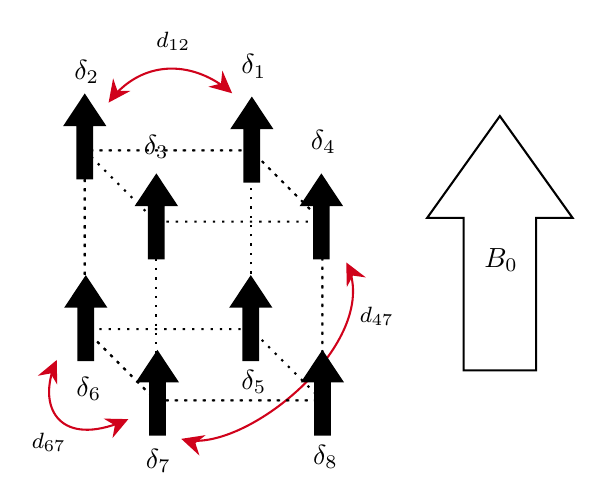
\begin{tikzpicture}[x=0.75pt,y=0.75pt,yscale=-1,xscale=1]
%uncomment if require: \path (0,300); %set diagram left start at 0, and has height of 300

%Up Arrow [id:dp8732081220560729] 
\draw  [fill={rgb, 255:red, 0; green, 0; blue, 0 }  ,fill opacity=1 ] (40,92.33) -- (49.5,78) -- (59,92.33) -- (53.03,92.33) -- (53.03,118) -- (45.97,118) -- (45.97,92.33) -- cycle ;
%Up Arrow [id:dp6011286918484611] 
\draw  [fill={rgb, 255:red, 0; green, 0; blue, 0 }  ,fill opacity=1 ] (74.5,130.83) -- (84,116.5) -- (93.5,130.83) -- (87.53,130.83) -- (87.53,156.5) -- (80.47,156.5) -- (80.47,130.83) -- cycle ;
%Up Arrow [id:dp7451953769890557] 
\draw  [fill={rgb, 255:red, 0; green, 0; blue, 0 }  ,fill opacity=1 ] (120.5,93.83) -- (130,79.5) -- (139.5,93.83) -- (133.53,93.83) -- (133.53,119.5) -- (126.47,119.5) -- (126.47,93.83) -- cycle ;
%Curve Lines [id:da42525692800879833] 
\draw [color={rgb, 255:red, 208; green, 2; blue, 27 }  ,draw opacity=1 ]   (34.72,208.59) .. controls (26.82,229.73) and (38.38,247.42) .. (68.17,235.01) ;
\draw [shift={(70.5,234)}, rotate = 515.56] [fill={rgb, 255:red, 208; green, 2; blue, 27 }  ,fill opacity=1 ][line width=0.08]  [draw opacity=0] (10.72,-5.15) -- (0,0) -- (10.72,5.15) -- (7.12,0) -- cycle    ;
\draw [shift={(36,205.5)}, rotate = 114.54] [fill={rgb, 255:red, 208; green, 2; blue, 27 }  ,fill opacity=1 ][line width=0.08]  [draw opacity=0] (10.72,-5.15) -- (0,0) -- (10.72,5.15) -- (7.12,0) -- cycle    ;
%Curve Lines [id:da4089633773753214] 
\draw [color={rgb, 255:red, 208; green, 2; blue, 27 }  ,draw opacity=1 ]   (99.24,244.21) .. controls (129.6,248.48) and (191.3,196.82) .. (176.5,160.69) ;
\draw [shift={(175.5,158.5)}, rotate = 423.13] [fill={rgb, 255:red, 208; green, 2; blue, 27 }  ,fill opacity=1 ][line width=0.08]  [draw opacity=0] (10.72,-5.15) -- (0,0) -- (10.72,5.15) -- (7.12,0) -- cycle    ;
\draw [shift={(96,243.5)}, rotate = 16.97] [fill={rgb, 255:red, 208; green, 2; blue, 27 }  ,fill opacity=1 ][line width=0.08]  [draw opacity=0] (10.72,-5.15) -- (0,0) -- (10.72,5.15) -- (7.12,0) -- cycle    ;
%Curve Lines [id:da6145675949482681] 
\draw [color={rgb, 255:red, 208; green, 2; blue, 27 }  ,draw opacity=1 ]   (62.85,79.13) .. controls (77.39,61.68) and (99.89,60.73) .. (118.23,75.12) ;
\draw [shift={(120.5,77)}, rotate = 221.07999999999998] [fill={rgb, 255:red, 208; green, 2; blue, 27 }  ,fill opacity=1 ][line width=0.08]  [draw opacity=0] (10.72,-5.15) -- (0,0) -- (10.72,5.15) -- (7.12,0) -- cycle    ;
\draw [shift={(61,81.5)}, rotate = 306.19] [fill={rgb, 255:red, 208; green, 2; blue, 27 }  ,fill opacity=1 ][line width=0.08]  [draw opacity=0] (10.72,-5.15) -- (0,0) -- (10.72,5.15) -- (7.12,0) -- cycle    ;
%Up Arrow [id:dp18329258081116873] 
\draw  [fill={rgb, 255:red, 0; green, 0; blue, 0 }  ,fill opacity=1 ] (154,130.83) -- (163.5,116.5) -- (173,130.83) -- (167.03,130.83) -- (167.03,156.5) -- (159.97,156.5) -- (159.97,130.83) -- cycle ;
%Up Arrow [id:dp8683108357041842] 
\draw  [fill={rgb, 255:red, 0; green, 0; blue, 0 }  ,fill opacity=1 ] (40.5,179.83) -- (50,165.5) -- (59.5,179.83) -- (53.53,179.83) -- (53.53,205.5) -- (46.47,205.5) -- (46.47,179.83) -- cycle ;
%Up Arrow [id:dp5759271994277898] 
\draw  [fill={rgb, 255:red, 0; green, 0; blue, 0 }  ,fill opacity=1 ] (75,215.83) -- (84.5,201.5) -- (94,215.83) -- (88.03,215.83) -- (88.03,241.5) -- (80.97,241.5) -- (80.97,215.83) -- cycle ;
%Up Arrow [id:dp9205895581383339] 
\draw  [fill={rgb, 255:red, 0; green, 0; blue, 0 }  ,fill opacity=1 ] (120,179.83) -- (129.5,165.5) -- (139,179.83) -- (133.03,179.83) -- (133.03,205.5) -- (125.97,205.5) -- (125.97,179.83) -- cycle ;
%Up Arrow [id:dp6721125512338199] 
\draw  [fill={rgb, 255:red, 0; green, 0; blue, 0 }  ,fill opacity=1 ] (154.5,215.83) -- (164,201.5) -- (173.5,215.83) -- (167.53,215.83) -- (167.53,241.5) -- (160.47,241.5) -- (160.47,215.83) -- cycle ;
%Shape: Cube [id:dp884827666481175] 
\draw  [dash pattern={on 0.84pt off 2.51pt}] (164,138.85) -- (129.65,104.5) -- (49.5,104.5) -- (49.5,190.65) -- (83.85,225) -- (164,225) -- cycle ; \draw  [dash pattern={on 0.84pt off 2.51pt}] (49.5,104.5) -- (83.85,138.85) -- (164,138.85) ; \draw  [dash pattern={on 0.84pt off 2.51pt}] (83.85,138.85) -- (83.85,225) ;
%Shape: Cube [id:dp10269830594110929] 
\draw  [dash pattern={on 0.84pt off 2.51pt}] (49.5,190.65) -- (83.85,225) -- (164,225) -- (164,138.85) -- (129.65,104.5) -- (49.5,104.5) -- cycle ; \draw  [dash pattern={on 0.84pt off 2.51pt}] (164,225) -- (129.65,190.65) -- (49.5,190.65) ; \draw  [dash pattern={on 0.84pt off 2.51pt}] (129.65,190.65) -- (129.65,104.5) ;
%Up Arrow [id:dp6620346842751581] 
\draw   (214.5,137) -- (249.5,88) -- (284.5,137) -- (267,137) -- (267,210.5) -- (232,210.5) -- (232,137) -- cycle ;

% Text Node
\draw (22.5,239.4) node [anchor=north west][inner sep=0.75pt]  [font=\footnotesize]  {$d_{67}$};
% Text Node
\draw (180.5,178.4) node [anchor=north west][inner sep=0.75pt]  [font=\footnotesize]  {$d_{47}$};
% Text Node
\draw (82.5,45.9) node [anchor=north west][inner sep=0.75pt]  [font=\footnotesize]  {$d_{12}$};
% Text Node
\draw (43,59.4) node [anchor=north west][inner sep=0.75pt]    {$\delta _{2}$};
% Text Node
\draw (76.5,95.9) node [anchor=north west][inner sep=0.75pt]    {$\delta _{3}$};
% Text Node
\draw (123.5,56.9) node [anchor=north west][inner sep=0.75pt]    {$\delta _{1}$};
% Text Node
\draw (157,93.4) node [anchor=north west][inner sep=0.75pt]    {$\delta _{4}$};
% Text Node
\draw (44,212.4) node [anchor=north west][inner sep=0.75pt]    {$\delta _{6}$};
% Text Node
\draw (77.5,246.9) node [anchor=north west][inner sep=0.75pt]    {$\delta _{7}$};
% Text Node
\draw (123.5,208.9) node [anchor=north west][inner sep=0.75pt]    {$\delta _{5}$};
% Text Node
\draw (158,244.9) node [anchor=north west][inner sep=0.75pt]    {$\delta _{8}$};
% Text Node
\draw (240.5,150.4) node [anchor=north west][inner sep=0.75pt]    {$B_{0}$};


\end{tikzpicture}
